%%*************************************************************************
%% The Berkeley Out-of-Order Machine
%% Christopher Celio
%% 2015 Dec 17
%% 
%% Design document
%%*************************************************************************


\documentclass[11pt, notitlepage]{report}


\usepackage{graphicx}
\usepackage{url}
\usepackage{fullpage}
\usepackage{listings}
\usepackage{color}
\usepackage[multiple]{footmisc}

\usepackage{hyperref}
\hypersetup{
    colorlinks=true,
    linkcolor=black,
    urlcolor=red,
    citecolor=black,
    filecolor=black,
    linktoc=all
}

\let\tt\texttt

\newcommand{\smalltodo}[1]{\marginpar{\footnotesize #1}}

\newcommand{\TODO}[1]{{\color{red} {\textbf [ TODO: #1 ]}}}
\newcommand{\fixme}[1]{{\color{red} {\textbf [ FIXME: #1 ]}}}
\newcommand{\ooo}{out-of-order}
\newcommand{\boom}{{\em BOOM}}
\newcommand{\BOOM}{{\em BOOM}}
\newcommand{\Chisel}{{\em Chisel}}
\newcommand{\Rocket}{{\em Rocket}}
\newcommand{\rocket}{{\em Rocket}}
\newcommand{\rocketchip}{{\em Rocket-chip}}


\let\oldthebibliography=\thebibliography
\let\endoldthebibliography=\endthebibliography
\renewenvironment{thebibliography}[1]{%
  \begin{oldthebibliography}{#1}%
    \setlength{\parskip}{0ex}%
    \setlength{\itemsep}{0ex}%
  }%
  {%
    \end{oldthebibliography}%
  }

%%*************************************************************************
\begin{document}


\title{The Berkeley Out-of-Order Machine (BOOM) Design Specification}
\author{Christopher Celio, David Patterson, and Krste Asanovi\'{c}\\
%School of Electrical and Computer Engineering\\
University of California, Berkeley, California 94720--1770\\
{\tt celio@eecs.berkeley.edu}}

\maketitle

%%*************************************************************************

\

\

{\centerline {\color{red}This draft is a work-in-progress.}}


\vfill

\hrule
\

\noindent The information in this publication is subject to change without notice. 

\noindent This document is available at: \url{https://github.com/ccelio/riscv-boom-doc}.

\

\noindent Copyright \copyright\ 2016 Christopher Celio

\

\noindent This work is licensed under the Creative Commons Attribution 4.0 International License (CC BY 4.0). To view a copy of this license, visit \url{http://creativecommons.org/licenses/by/4.0/}.


\thispagestyle{empty} % suppress page number 

%%*************************************************************************

\tableofcontents


\chapter{Introduction \& Overview}
\label{sec:introduction}

The goal of this document is to describe the design and implementation of the Berkeley Out--of--Order Machine (BOOM). 


 BOOM is heavily inspired by the MIPS R10k and the Alpha 21264 out--of--order processors\cite{alpha21264, mipsr10k}.  Like the R10k and the 21264, BOOM is a unified physical register file design (also known as ``explicit register renaming"). 
 
 The source code to BOOM can be found at (\url{https://ucb-bar.github.io/riscv-boom}).

\section{The BOOM Pipeline}


\begin{figure}[ht]
	\centering
	\centerline{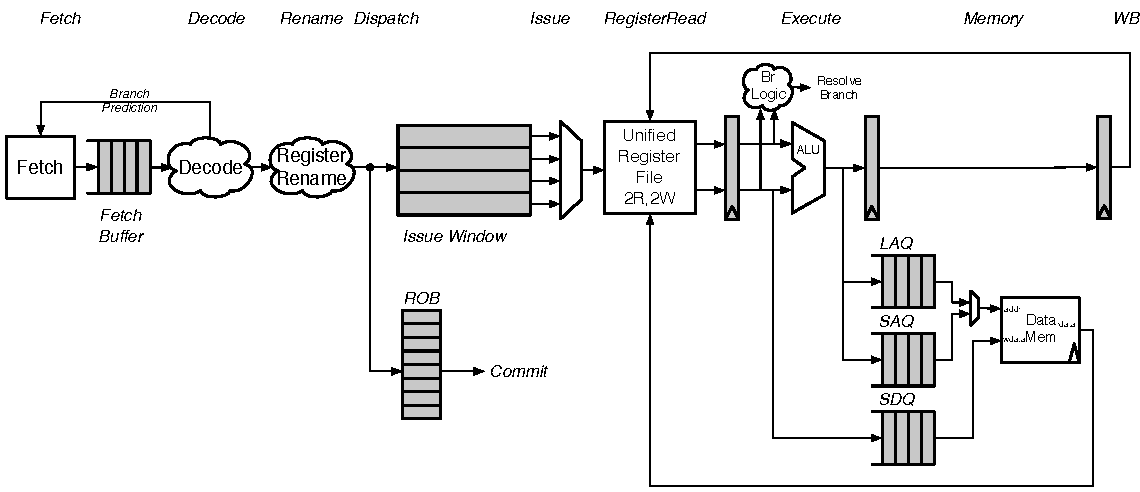
\includegraphics[scale =.9] {figures/boom_stages}}
	\caption{ \small The Berkeley Out of Order Machine Processor.}
	\label{fig:boom_stages}
\end{figure}



Conceptually, BOOM is broken up into 10 stages: {\em Fetch, Decode, Register Rename, Dispatch, Issue, Register Read, Execute, Memory, Writeback,} and {\em Commit}.  However, many of those stages are combined in the current implementation, yielding {\em six} stages: {\em Fetch, Decode/Rename/Dispatch, Issue/RegisterRead, Execute, Memory,} and {\em Writeback} ({\em Commit} occurs asynchronously, so I'm not counting that as part of the ``pipeline").   

\begin{quote}
\begin{description}
\item[Fetch]  Instructions are {\em fetched} from the Instruction Memory and placed into a FIFO queue, known as the {\em fetch buffer}.\footnote{While the fetch buffer is N-entries deep, it can instantly read out the first instruction on the front of the FIFO.  Put another way, instructions don't need to spend N cycles moving their way through the {\em fetch buffer} if there are no instructions in front of them.}
\item[Decode]
{\em Decode} pulls instructions out of the {\em fetch buffer} and generates the appropriate ``micro-op" to place into the pipeline.\footnote{Because RISC-V is a RISC ISA, currently all instructions generate only a single micro-op. More details on how store micro-ops are handled can be found in Chapter \ref{chapter:memory}.} 

\item[Rename]
 The ISA, or ``logical", register specifiers are then {\em renamed} into ``physical" register specifiers.
  
\item[Dispatch] The instruction is then {\em dispatched}, or written, into the {\em Issue Window}.  
 
\item[Issue]   Instructions sitting in the {\em Issue Window} wait until all of their operands are ready, and are then {\em issued}.\footnote{More precisely, uops that are ready assert their request, and the issue scheduler chooses which uops to issue that cycle.}  This is the beginning of the out--of--order piece of the pipeline.
\item[RF Read]  Issued instructions first {\em read} their operands from the unified physical register file (or from the bypass network)... 
\item[Execute] and then enter the {\em Execute} stage where the functional units reside.  Issued memory operations perform their address calculations in the {\em Execute} stage, and then store the calculated addresses in the Load/Store Unit which resides in the {\em Memory} stage.  
 
\item[Memory]  The Load/Store Unit consists of three queues: a Load Address Queue (LAQ), a Store Address Queue (SAQ), and a Store Data Queue (SDQ).  Loads are fired to memory when their address is present in the queue and does not conflict with any of the store addresses that the load depends on. Stores are fired to memory at commit time, when both its address and its data are present.  
 
\item[Writeback]  ALU operations and load operations are {\em written} back to the physical register file.
\item[Commit] The Reorder Buffer, or ROB, tracks the status of each instruction in the pipeline.  When the head of the ROB is not-busy, it {\em commits} the instruction.  For stores, the ROB signals to the store at the head of the Store Queue that it can now write its data to memory.
\end{description}
\end{quote}


  
BOOM supports full branch speculation and branch prediction.  Each instruction, no matter where it is in the pipeline,  is accompanied by a branch tag that marks which branches the instruction is ``speculated under". A mispredicted branch requires killing all instructions that depended on that branch.  When a branch instructions passes through {\em Rename}, copies of the {\em Register Rename Table} and the {\em Free List} are made.  On a mispredict, the saved processor state is restored.

Although Figure \ref{fig:boom_stages} shows a simplified pipeline, BOOM implements the RV64G and privileged ISAs, which includes single- and double-precision floating point, atomic memory support, and page-based virtual memory. 



\section{The RISC-V ISA}

BOOM implements the RV64G variant of the RISC-V ISA. This includes the MAFD
extensions and the privileged specification (multiply/divide, AMOs,
load-reserve/store-conditional, single- and double-precision IEEE
754-2008 floating point). More information about the RISC-V
ISA can be found at (\url{http://riscv.org}).

RISC-V provides the following features which make it easy to target with high-performance designs:

\begin{quote}
\begin{description}
\item [Relaxed memory model] This greatly simplifies the Load/Store Unit, which does not need to have loads snoop other loads nor does coherence traffic need to snoop the LSU, as required by sequential consistency.
\item [accrued floating point exception flags] The fp status register does not need to be renamed, nor can FP instructions throw exceptions themselves. 
\item [no integer side-effects] All integer ALU operations exhibit no side-effects, save the writing of the destination register. This prevents the need to rename additional condition state.
\item [no \bf{cmov} or predication] Although predication can lower the branch predictor complexity of small designs, it greatly complicates OoO pipelines, including the addition of a third read port for integer operations.
\item [no implicit register specifiers] Even JAL requires specifying an explicit \tt{rd}. This simplifies rename logic, which prevents either the need to know the instruction first before accessing the rename tables, or it prevents adding more ports to remove the instruction decode off the critical path.
\item [\tt{rs1}, \tt{rs2}, \tt{rs3}, \tt{rd} are always in the same place] This allows decode and rename to proceed in parallel. 

\end{description}
\end{quote}

BOOM (currently) does not implement the ``C" compressed extension nor the ``V" vector extension.

\section{The \Chisel\ Hardware Construction Language}

BOOM is implemented in the \Chisel\ hardware construction language.  More information about \Chisel\ can be found at (\url{http://chisel.eecs.berkeley.edu}). 

\newpage

\section{Quick-start}


To build a BOOM C++ emulator and run BOOM through a couple of simple tests:
\\

\texttt{\$} \verb=export ROCKETCHIP_ADDONS==\verb="boom"=

\texttt{\$} \verb=git clone https://github.com/ucb-bar/rocket-chip.git=

\texttt{\$} \verb=cd rocket-chip=

\texttt{\$} \verb=git checkout boom=

\texttt{\$} \verb=git submodule update --init=

\texttt{\$} \verb=cd riscv-tools=

\texttt{\$} \verb=git submodule update --init --recursive riscv-tests=

\texttt{\$} \verb=cd ../emulator; make run CONFIG==\verb=BOOMCPPConfig=

\

{\bf Note:} this assumes you have already installed the riscv-tools toolchain.  If not, visit (\url{https://github.com/riscv/riscv-tools}).

\section{The BOOM Repository}

The BOOM repository holds the source code to the BOOM core; it is not a full processor and thus is \textbf{NOT A SELF-RUNNING} repository.  To instantiate a BOOM core, the Rocket chip generator found in the rocket-chip git repository must be used (\url{https://github.com/ucb-bar/rocket-chip}), which provides the caches, uncore, and other needed infrastructure to support a full processor.

The BOOM source code can be found in \verb=boom/src/main/scala=.  

The code structure is shown below:

\begin{quote}
\begin{itemize}
\item \verb=boom/src/main/scala=/\begin{itemize}
  \item bpd\_pipeline.scala {\footnotesize \color{red} branch prediction stage.}
  \item brpredictor.scala {\footnotesize \color{red} abstract branch predictor.}
  \item configs.scala {\footnotesize \color{red} BOOM configurations. }
  \item consts.scala {\footnotesize \color{red} constant definitions. }
  \item core.scala {\footnotesize \color{red} the top-level of the processor core.}
  \item dcacheshim.scala {\footnotesize \color{red} the shim between the the core and the dcache.}
  \item decode.scala {\footnotesize \color{red} decode stage.}
  \item dpath.scala {\footnotesize \color{red} core datapath.}
  \item execute.scala {\footnotesize \color{red} high-level execution units (made up of FUs).}
  \item fpu.scala {\footnotesize \color{red} floating point unit.}
  \item functional\_unit.scala {\footnotesize \color{red} low-level functional units.}
  \item gshare.scala {\footnotesize \color{red} gshare branch predictor.}
  \item imul.scala {\footnotesize \color{red} integer multiplier.}
  \item issue\_ageordered.scala {\footnotesize \color{red} age-ordered (collasping-queue) issue window implementation.}
  \item issue.scala {\footnotesize \color{red} abstract issue window.}
  \item issue\_slot.scala {\footnotesize \color{red} An issue window slot.}
  \item issue\_unordered.scala {\footnotesize \color{red} un-ordered issue window implementation.}
  \item lsu.scala {\footnotesize \color{red} load/store unit.}
  \item package.scala {\footnotesize \color{red} }
  \item parameters.scala {\footnotesize \color{red} knobs/parameters.}
  \item prefetcher.scala {\footnotesize \color{red} data prefetcher.}
  \item regfile.scala {\footnotesize \color{red} register file.}
  \item registerread.scala {\footnotesize \color{red} registerRead stage and bypassing.}
  \item rename.scala {\footnotesize \color{red} register renaming logic.}
  \item rob.scala {\footnotesize \color{red} re-order buffer.}
  \item tile.scala {\footnotesize \color{red} top-level tile.}
  \item util.scala {\footnotesize \color{red} utility code.}


\end{itemize}
\end{itemize}
\end{quote}




\section{The Rocket-chip Repository Layout}

As BOOM is just a core, an entire SoC infrastructure must be provided.  BOOM was developed to use the open-source Rocket-chip SoC generator (\url{https://github.com/ucb-bar/rocket-chip}). The Rocket-chip generator can instantiate a wide range of SoC designs, including cache-coherent multi-tile designs, cores with and without accelerators, and chips with or without a last-level shared cache. 




\begin{figure}[ht]
	\centering
	\centerline{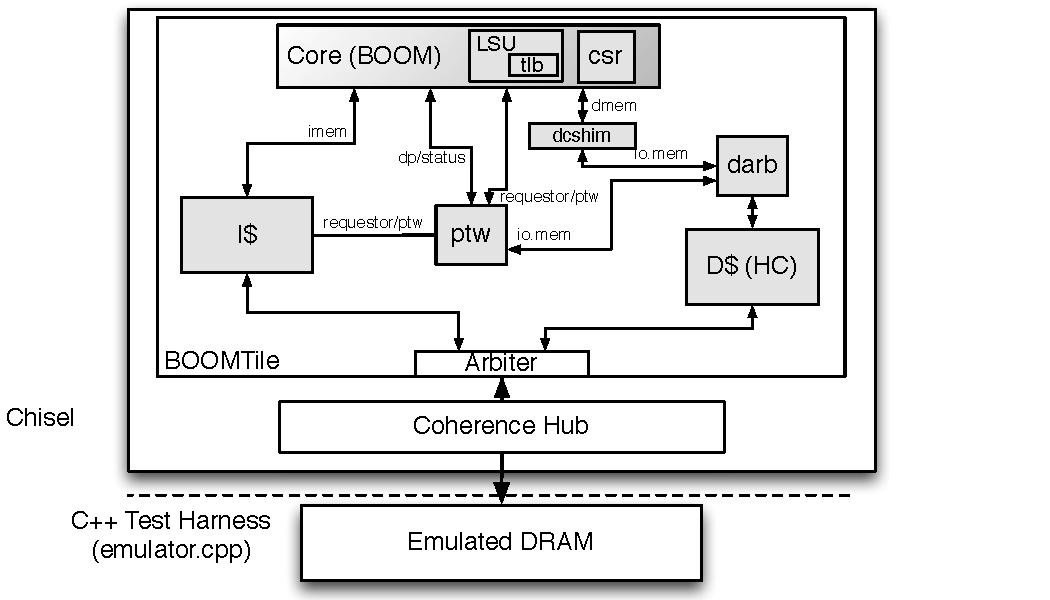
\includegraphics[scale =.9] {figures/chip}}
	\caption{ \small A single-core ``BOOM-chip", with no L2 last-level cache.}
	\label{fig:boomchip}
\end{figure}



To manage the wide array of actively developed projects that encompass Rocket-chip, the Rocket-chip repository makes heavy use of git submodules. The directory structure of the Rocket-chip repository is shown below. 

\begin{quote}
\begin{itemize}
\item \verb=rocket-chip=/\begin{itemize}

  \item boom/ {\footnotesize \color{red} Git submodule of the \Chisel\ source code for the BOOM core.}
  \item chisel {\footnotesize \color{red}  The source code to the {\tt Chisel} language itself.}
  \item csrc/ {\footnotesize \color{red} Utility C/C++ source code.}
  \item dramsim2/ {\footnotesize \color{red} Git submodule of a C++ DRAM emulator.}
  
  \item emulator/ {\footnotesize \color{red} C++ simulation tools and support.}\begin{itemize}
    \item generated-src/{\footnotesize \color{red} Auto-generated C++ code.} 
    \item Makefile {\footnotesize \color{red} Makefile for C++ simulation.}
    \item output/{\footnotesize \color{red} Output files from C++ simulation runs.} 
    \end{itemize}
  \item fpga-zynq/ {\footnotesize \color{red} Git submodule of the zynq FPGA tools.}
  \item fsim/ {\footnotesize \color{red} The FPGA Verilog simulation and build directories. }
  \item junctions/ {\footnotesize \color{red} Git submodule of the \Chisel\ source code for the uncore and off-chip network.}
 \item riscv-tools/{\footnotesize \color{red} Git submodule that points to the RISC-V toolchain.}
 \begin{itemize} 
  \item riscv-tests/ {\footnotesize \color{red} Source code for benchmarks and tests.} \begin{itemize}
    \item riscv-bmarks/ {\footnotesize \color{red}  Benchmarks written in C.}
    \item riscv-tests/ {\footnotesize \color{red}  Tests written in assembly.}
  \end{itemize}
  \end{itemize}
   \item Makefrag {\footnotesize \color{red}  The high-level Makefile fragment.}
   
  \item src/ {\footnotesize \color{red} \Chisel\ source code for top-level Rocket-chip.}
  \item rocket/ {\footnotesize \color{red} Git submodule of the \Chisel\ source code for the Rocket core (used as a library of processor components).}
      \item sbt/ {\footnotesize \color{red} {\tt Chisel}/Scala voodoo.}
  \item uncore/ {\footnotesize \color{red} Git submodule of the \Chisel\ source code for the uncore components (including LLC).}
    \item vsim/ {\footnotesize \color{red} The ASIC Verilog simulation and build directories. }
    \item zscale/ {\footnotesize \color{red} Git submodule of the \Chisel\ source code for the zscale micro-controller core. }
   
\end{itemize}
\end{itemize}
\end{quote}

\subsection{The Rocket Core - a Library of Processor Components!}\label{sec:rocket}

Rocket is a 5-stage in-order core that implements the RV64G ISA and page-based virtual memory.  The original design purpose of the Rocket core was to enable architectural research into vector co-processors by serving as the scalar {\em Control Processor}.  Some of that work can be found at (\url{http://hwacha.org}). 

Rocket has been taped out at least ten times in two different commercial processes, and has been successfully demonstrated to reach over 1.65 GHz in IBM 45 nm SOI.\cite{riscv_nature} As its namesake suggests, Rocket is the baseline core for the Rocket-chip SoC generator. As discussed earlier, BOOM is instantiated by replacing a Rocket tile with a BOOM tile. 

However, from BOOM's point of view, Rocket can also be thought of as a ``Library of Processor Components."  There are a number of modules created for Rocket that are also used by BOOM - the functional units, the caches, the translation look-aside buffers, the page table walker, and more.  Thus, throughout this document you will find references to these Rocket components and descriptions on how they fit into BOOM.

The source code to Rocket can be found at (\url{https://github.com/ucb-bar/rocket}).  


\chapter {Instruction Fetch}

Figure \ref{fig:fetch} shows the Fetch Unit organization used by BOOM. 

\begin{figure}[ht]
	\centering
	\centerline{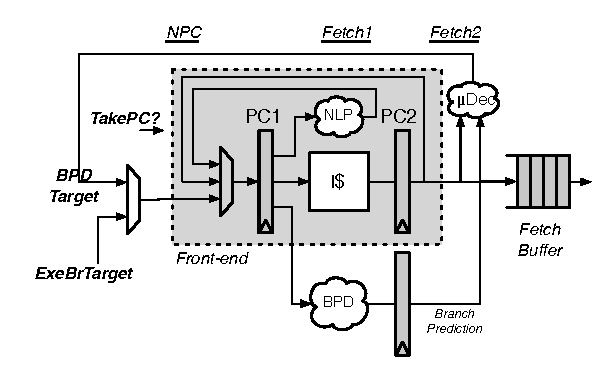
\includegraphics[scale =1] {figures/frontend}}
	\caption{ \small The Fetch Unit. The grey box is the front-end instantiated from the Rocket code base.}
	\label{fig:fetch}
\end{figure}

BOOM instantiates the Rocket core's {\em Front-end} (highlighted in grey in Fig \ref{fig:fetch}), which fetches instructions and predicts every cycle where to fetch the next instructions using a ``next-line predictor" (NLP). If a misprediction is detected in BOOM's backend, or BOOM's own predictor wants to redirect the pipeline in a different direction, a request is sent to the Front-End and it begins fetching along a new instruction path.  See Chapter \ref{chapter:bpd} for more information on how branch prediction fits into the Fetch Unit's pipeline. 

As superscalar fetch is supported, the {\em Front-end} returns a {\em fetch packet} of instructions.  The {\em fetch packet} also contains meta-data, which includes a {\em valid mask} (which instructions in the packet are valid?) and some branch prediction information that is used later in the pipeline. 

\section{The Rocket I-Cache}

BOOM instantiates the i-cache found in the Rocket processor source code.  The i-cache is a virtually indexed, physically tagged set-associative cache. 

To save power, the i-cache reads out a fixed number of bytes (aligned) and stores the instruction bits into a register. Further instruction fetches can be managed by this register. The i-cache is only fired up again once the fetch register has been exhausted (or a branch prediction directs the PC elsewhere).  

The i-cache does not (currently) support fetching across cache-lines, nor does it support fetching unaligned relative to the superscalar fetch address.


The i-cache does not (currently) support hit-under-miss.  If an icache miss occurs, the icache will not accept any further requests until the miss has been handled.  This is less than ideal for scenarios in which the pipeline discovers a branch mispredict and would like to redirect the icache to start fetching along the correct path. 

%When a miss occurs, the cache-line is returned in smaller chunks over a parameterizable N refill cycles. The size of a refill chunk dictates the width of the instantiated memory bank. Thus, within a way, a cache-line is striped across the physical memory bank to match the incoming refill size. To minimize power, at most only one row of the memory bank is read a cycle, which dictates the maximum size of the fetch register. Thus, the i-cache (currently) does not support fetching instruction packets that straddle across a memory bank row.  Worded another way, if BOOM is parameterized to have 64 byte cache lines and the uncore returns 16 bytes per cycle over 4 cycles, 


The front-end (currently) only handles the RV64G ISA, which uses fixed-size 4 bytes instructions. 

\section{The Fetch Buffer}

{\em Fetch packets} coming from the i-cache are placed into a {\em Fetch Buffer}.  The {\em Fetch Buffer} helps to decouple the instruction fetch front-end from the execution pipeline in the back-end. 

The instructions within a {\em fetch packet} are {\em not} collapsed or compressed - any bubbles within a {\em fetch packet} are maintained. 

The {\em Fetch Buffer} is parameterizable. The number of entries can be changed and whether the buffer is implemented as a ``flow-through" queue\footnote{A flow-through queue allows entries being enqueued to be immediately dequeued if the queue is empty and the consumer is requesting (the packet ``flows through" instantly).} or not can be toggled.  
 
\chapter{Branch Prediction}\label{chapter:bpd}

This chapter discusses how BOOM predicts branches and then resolves these predictions.

BOOM uses two levels of branch prediction- a single-cycle ``next-line predictor" (NLP), and a slower but more complex ``backing predictor" (BPD).\footnote{Unfortunately, the terminology in the literature gets a bit muddled here in what to call different types and levels of branch predictor. I have seen ``micro-BTB" versus ``BTB", ``NLP" versus ``BHT", and ``cache-line predictor" versus ``overriding predictor". 
Although the Rocket code calls its own predictor the ``BTB", I have chosen to refer to it in documentation as the ``next-line predictor", to denote that it is a combinational predictor that provides single-cycle predictions for fetching ``the next line", and the Rocket BTB encompasses far more complexity than just a ``branch target buffer" structure.  Likewise, I have chosen the name ``backing predictor" as I believe it is the most accurate name, while simultaneously avoiding being overly descriptive of the internal design (is it a simple BHT? Is it tagged? Does it override the NLP?).
{\color{red} But in short, I am open to better names!}}



\begin{figure}[ht]
	\centering
	\centerline{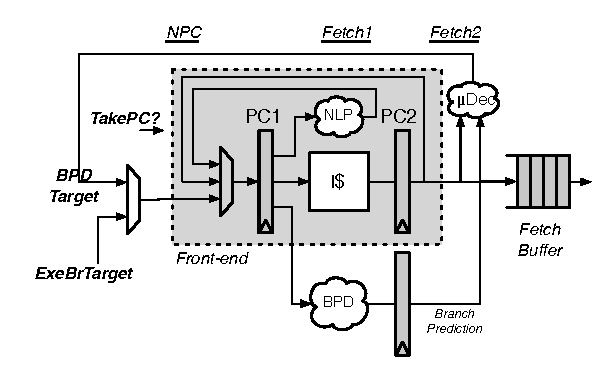
\includegraphics[scale =1] {figures/frontend}}
	\caption{ \small The Fetch Unit.}
	\label{fig:fetch}
\end{figure}


\section{The Rocket Next-line Predictor (NLP)}

BOOM instantiates the Rocket core's Front-End, which fetches instructions and predicts every cycle where to fetch the next instructions. If a misprediction is detected in BOOM's backend, or BOOM's own backing predictor wants to redirect the pipeline in a different direction, a request is sent to the Front-End and it begins fetching along a new instruction path. 

The next-line predictor (NLP) takes in the current PC being used to fetch instructions (the {\em Fetch PC}) and predicts combinationally where the next instructions should be fetched for the next cycle. If predicted correctly, there are no pipeline bubbles. 

The next-line predictor is an amalgamation of a fully-associative branch target buffer (BTB), a {\em gshare} branch history table (BHT), and a return address stack (RAS) which work together to make a fast, but reasonably accurate prediction.

\subsection{NLP Predictions}

The {\em Fetch PC} first performs a tag match to find a uniquely matching BTB entry.  
If a hit occurs, the BTB entry will make a prediction in concert with the BHT and RAS as to whether there is a branch, jump, or return found in the {\em fetch packet} and which instruction in the {\em fetch packet} is to blame.  
The BTB entry also contains a predicted PC target, which is used as the {\em Fetch PC} on the next cycle.

\TODO{add an image showing how the BTB stores data, and makes predictions}


The hysteresis bits (governed by a {\em gshare} predictor) are only used on a BTB entry {\em hit} and if the predicting instruction is a branch.

If the BTB entry contains a {\em return} instruction, the RAS stack is used to provide the predicted return PC as the next {\em Fetch PC}. The actual RAS management (of when to {\tt {pop}} or {\tt {push}} the stack) is governed externally. 

For area-efficiency, the high-order bits of the PC tags and PC targets are stored in a compressed file.


\subsection{NLP Updates}

Each branch passed down the pipeline remembers not only its own PC, but also its {\em Fetch PC} (the PC of the head instruction of its {\em fetch packet}).\footnote{In reality, only the very lowest bits must be saved, as the higher-order bits will be the same.}  



\subsubsection{BTB Updates}

The BTB is updated {\bf only} when the Fetch Unit is redirected to {\bf take} a branch or jump by either the Branch Unit (in the {\em Execute} stage) or the Backing Predictor (in the {\em Branch Predict} stage).\footnote{Rocket's BTB relies on a little cleverness - when redirecting the PC on a misprediction, this new {\em Fetch PC } is the same as the {\em Update PC} that needs to be written into a new BTB entry's {\em Target PC} field. This ``coincidence" allows the PC compression table to use a single search port - it is simultaneously reading the table for the next prediction while also seeing if the new {\em Update PC} already has the proper high-order bits allocated for it.}

If there is no BTB entry corresponding to the taken branch or jump, an new entry is allocated for it.

\subsubsection{BHT Updates}

The BHT is composed of two parts that require updates - a {\em global history (ghistory)} register and a table of {\em history counters}. 

The \ghistory\ register tracks the outcomes of the last $N$ branches that have been fetched. It must be updated:

\begin{itemize}
\item in the {\em Branch Predict} stage - once we have decoded the instruction {\em fetch bundle}, know if any branches are present, and which direction the branch predictors have chosen to direct the Fetch Unit.
\item in the {\em Execute} stage - if and only if a {\em misprediction} occurs, the \ghistory\ register must be reset with the correct outcome of the branch history.
\end{itemize}

The {\em history counter} table is updated when the \ghistory\ register is updated.  Because the counters are read out and passed down the pipeline with the branch instruction, there is not a problem with having updated the counters incorrectly in the earlier {\em Branch Predict} stage. If a misprediction occurs, the counters will be reset and incremented to the proper value.

Notice that by updating the history counters in the {\em Branch Predict} stage, the updates are being performed in-order!  However, it is possible for a branch to update the {\em history counters} before later being found to have been misspeculated under a previous branch. We suspect that this is a fairly benign scenario.\footnote{Likewise, the BHT does not keep track of a {\em commit copy} of the \ghistory\ register.  This means that any sort of exceptions or pipeline replays will leave the \ghistory\ register in an incoherent state.  However, experiments showed that this had no noticeable effect on performance on real benchmarks.  This is probably because the BHT's \ghistory\ register is fairly small and can quickly re-learn the history in only a few cycles.}


\subsubsection{RAS Updates}

The RAS is updated during the {\em Branch Predict} stage once the instructions in the {\em fetch packet} have been decoded. If the taken instruction is a call\footnote{While RISC-V does not have a dedicated {\tt {CALL}} instruction, it can be inferred by checking for a {\tt {JAL}} or {\tt {JALR}} instruction with a writeback destination to {\tt {x1}} (aka, the {\tt {return address register}}).}, the {\em Return Address} is {\tt {pushed}} onto the RAS. If the taken instruction is a {\tt {RETURN}}, then the RAS is {\tt {popped}}.

\



When the NLP makes a prediction, it is actually using the BTB to tag match against the predicted branch's {\em Fetch PC}, and not the PC of the branch itself.  
The NLP must predict across the entire {\em fetch packet} which of the many possible branches will be the dominating branch that redirects the PC.
For this reason, we use a given branch's {\em Fetch PC} rather than its own PC in the BTB tag match.\footnote{Each BTB entry corresponds to a single {\em Fetch PC}, but it is helping to predict across an entire {\em fetch packet}. However, the BTB entry can only store meta-data and target-data on a single control-flow instruction.  While there are certainly pathological cases that can harm performance with this design, the assumption is that there is a correlation between which branch in a {\em fetch packet} is the dominating branch relative to the {\em Fetch PC}, and - at least for narrow fetch designs - evaluations of this design has shown it is very complexity-friendly with no noticeable loss in performance. Some other designs instead choose to provide a whole bank of BTBs for each possible instruction in the {\em fetch packet}.} 

\section{The Backing Predictor (BPD)}

When the next-line predictor (NLP) is predicting well, the processor's backend is provided an unbroken stream of instructions to execute. The NLP is able to provide fast, single-cycle predictions by being expensive (in terms of both area and power), very small (only a few dozen branches can be remembered), and very simple (the {\em gshare} hysterisis bits are not able to learn very complicated or long history patterns).

To capture more branches and more complicated branching behaviors, BOOM provides support for a ``Backing Predictor", or BPD. 

The BPD's goal is to provide very high accuracy in a (hopefully) dense area.  To make this possible, the BPD will not make a prediction until the {\em fetch packet} has been decoded and the branch targets computed directly from the instructions themselves.  This saves on needing to store the {\em PC tags} and {\em branch targets} within the BPD.\footnote{It's the {\em PC tag} storage and {\em branch target} storage that makes the BTB within the NLP so expensive.}

The BPD is accessed in parallel with the instruction cache access (See Fig. \ref{fig:fetch}).  This allows the BPD to be stored in sequential memory (i.e., SRAM instead of flip-flops). With some clever designing, the BPD can be stored in single-ported SRAM to achieve the density desired.\cite{ev8}

\subsection{Making Predictions}

When making a prediction, the backing predictor must provide the following:

\begin{itemize}
\item is a prediction being made?
\item a bit-vector of taken/not-taken predictions
\end{itemize}

As per the first bullet-point, the BPD may decide to not make a prediction. This may be because the predictor uses tags to inform whether its prediction is valid or there may be a structural hazard that prevented a prediction from being made.

The BPD provides a bit-vector of taken/not-taken predictions, the size of the bit-vector matching the {\em fetch width} of the pipeline. The {\em Branch Prediction} stage will decode the instructions in the {\em fetch packet}, compute the branch targets, and decide in conjunction with the BPD's prediction bit-vector if a Front End redirect should be made. 

\subsubsection{Jump and Jump-Register Instructions}

The BPD makes predictions only on the direction (taken versus not-taken) of conditional branches.  Non-conditional ``jumps" (\jal) and ``jump-register" (\jalr) instructions are handled separately from the BPD.\footnote{\jal\ instructions jump to a $PC+Immediate$ location, whereas \jalr\ instructions jump to a $PC+Register[rs1]+Immediate$ location.}

The NLP learns any ``taken" instruction's {\em PC} and {\em target PC} - thus, the NLP is able to predict jumps and jump-register instructions.

If the NLP does not make a prediction on a \jal\ instruction, the pipeline will redirect the Fetch Unit in the {\em Fetch2 Stage} (see Fig. \ref{fig:fetch}).\footnote{Redirecting the Fetch Unit in the {\em Fetch2 Stage} for \jal\ instructions is trivial, as the instruction can be decoded and its target can be known.}

Jump-register instructions that were not predicted by the NLP will be sent down the pipeline with no prediction made.  As \jalr\ instructions require reading the register file to deduce the jump target, there's nothing that can be done if the NLP does not make a prediction.


\subsection{Updating the Backing Predictor}

Generally speaking, the BPD is updated during the {\em Commit} stage. This prevents the BPD from being polluted by wrong-path information.\footnote{In the data-cache, it can be useful to fetch data from the wrong path- it is possible that future code executions may want to access the data. Worst case, the cache's effective capacity is reduced. But it can be quite dangerous to add wrong-path information to the BPD - it truly represents a code-path that is never exercised, so the information will {\em never} be useful in later code executions. Worst, aliasing is a problem in branch predictors (at most partial tag checks are used) and wrong-path information can create deconstructive aliasing problems that worsens prediction accuracy.  Finally, bypassing of the inflight prediction information can occur, eliminating any penalty of not updating the predictor until the {\em Commit} stage.}  
However, as the BPD makes use of global history, this history must be reset whenever the Fetch Unit is redirected. Thus, the BPD must also be (partially) updated during {\em Execute} when a misprediction occurs to reset any speculative updates that had occurred during the {\em Fetch} stages.



%When making a prediction, the BPD passes to the pipeline a ``response info packet".  This ``info packet" is stored in a ``branch re-order buffer" (BROB) until commit time.\footnote{These {\em info packets} are not stored in the ROB for two reasons - first, they correspond to {\em fetch packets}, not instructions.  Second, they are very expensive and so it is reasonable to size the BROB to be smaller than the ROB.}  Once all of the instructions corresponding to the ``info packet" is committed, the ``info packet" is set to the BPD (along with the eventual outcome of the branches) and the BPD is updated. 

\subsection{Managing the Global History Register}

The {\em global history register} is an important piece of a branch predictor. It contains the outcomes of the previous $N$ branches (where $N$ is the size of the global history register).\footnote{Actually, the direction of all conditional branches within a {\em fetch packet} are compressed (via an OR-reduction) into a single bit, but for this section, it is easier to describe the history register in slightly inaccurate terms.}

When fetching branch $i$, it is important that the direction of the previous $i-N$ branches is available so an accurate prediction can be made.  Waiting till the {\em Commit} stage to update the global history register would be too late (dozens of branches would be inflight and not reflected!). Therefore, the global history register must be updated {\em speculatively}, once the branch is fetched and predicted in the {\em BP2} stage.

If a misprediction occurs, the global history register must be reset and updated to reflect the actual history.  This means that each branch (more accurately, each {\em fetch packet}) must snapshot the global history register in case of a misprediction.

There is one final wrinkle - exceptional pipeline behavior.  While each branch contains a snapshot of the global history register, any instruction can potential throw an exception that will cause a Front End redirect. Such an event will cause the global history register to become corrupted. For exceptions, this may seem acceptable - exceptions should be rare and the trap handlers will cause a pollution of the global history register anyways (from the point of view of the user code).  However, some exceptional events include ``pipeline replays" - events where an instruction causes a pipeline flush and the instruction is refetched and re-executed.\footnote{An example of a pipeline replay is a {\em memory ordering failure} in which a load executed before an older store it depends on, and got the wrong data. The only recovery requires flushing the entire pipeline and re-executing the load.}  For this reason, a {\em commit copy} of the global history register is also maintained by the BPD and reset on any sort of pipeline flush event.

\subsection{The Abstract Branch Predictor Class}

To facilitate exploring different global history-based BPD designs, an abstract ``BrPredictor" class is provided.  It provides a standard interface into the BPD, the control logic for managing the global history register, and contains the {\em branch reorder buffer (BROB)} (which handles the inflight branch prediction checkpoints).

\subsubsection{The Branch Reorder Buffer (BROB)}

\TODO{...}

\subsubsection{Global History}

\TODO{...}

\subsection{The GShare Predictor}

\TODO{...}

\subsection{The TAGE Predictor}

\TODO{...}

\subsection{Other Predictors}

BOOM provides a number of other predictors that may provide useful.

\subsubsection{The Null Predictor}

The Null Predictor is used when no BPD predictor is desired. It will always predict ``not taken".

\subsubsection{The Random Predictor}

The Random Predictor uses an LFSR to randomize both ``was a prediction made?" and ``which direction each branch in the {\em fetch packet} should take?".  This is very useful for both torturing-testing BOOM and for providing a worse-case performance baseline for comparing branch predictors.

\section{Branch Prediction Configurations}

There are a number of parameters provided to govern the branch prediction in BOOM.

\TODO{...}
 

\chapter{The Decode Stage}

The decode stage takes instructions from the fetch buffer, decodes them, and allocates the necessary resources as required by each instruction.  The decode stage will stall as needed if not all resources are available.

%\TODO{discuss parameterization, and the coupling of fetch width to decode width}.

%\TODO{discuss allocating branch tags and branch mask bits and other resources?}
\chapter{The Rename Stage}

The rename stage maps the {\em ISA} (or {\em logical}) register specifiers of each instruction to {\em physical} register specifiers. 

% discuss how this is an explicit renamed design
% discuss what renaming gets us (breaks all but true dependences)
% allows loop iterations to procceed in parallel, thanks to breaking the ``name" hazard

\section{The Purpose of Renaming}

{\em Renaming} is a technique to rename the ISA (or {\em logical}) register specifiers in an instruction by mapping them to a new space of {\em physical} registers.  The goal to {\em register renaming} is to break the output- (WAW) and anti-dependences (WAR) between instructions, leaving only the true dependences.  Said again, but in architectural terminology, register renaming eliminates write-after-write (WAW) and write-after-read (WAR) hazards, which are artifacts introduced by a) only having a limited number of ISA registers to use as specifiers and b) loops, which by their very nature will use the same register specifiers on every loop iteration. 

\section{The Explicit Renaming Design}

BOOM is an ``explicit renaming" or ``physical register file" out-of-order core design.  A physical register file, containing many more registers than the ISA dictates, holds both the committed architectural register state and speculative register state. The rename map tables contain the information needed to recover the committed state. As instructions are renamed, their register specifiers are explicitly updated to point to physical registers located in the physical register file. The MIPS R10k, Alpha 21264, Intel Sandy Bridge, and ARM Cortex A15 cores are all example of explicit renaming out-of-order cores. 


\begin{figure}[htb]
	\centering
	\centerline{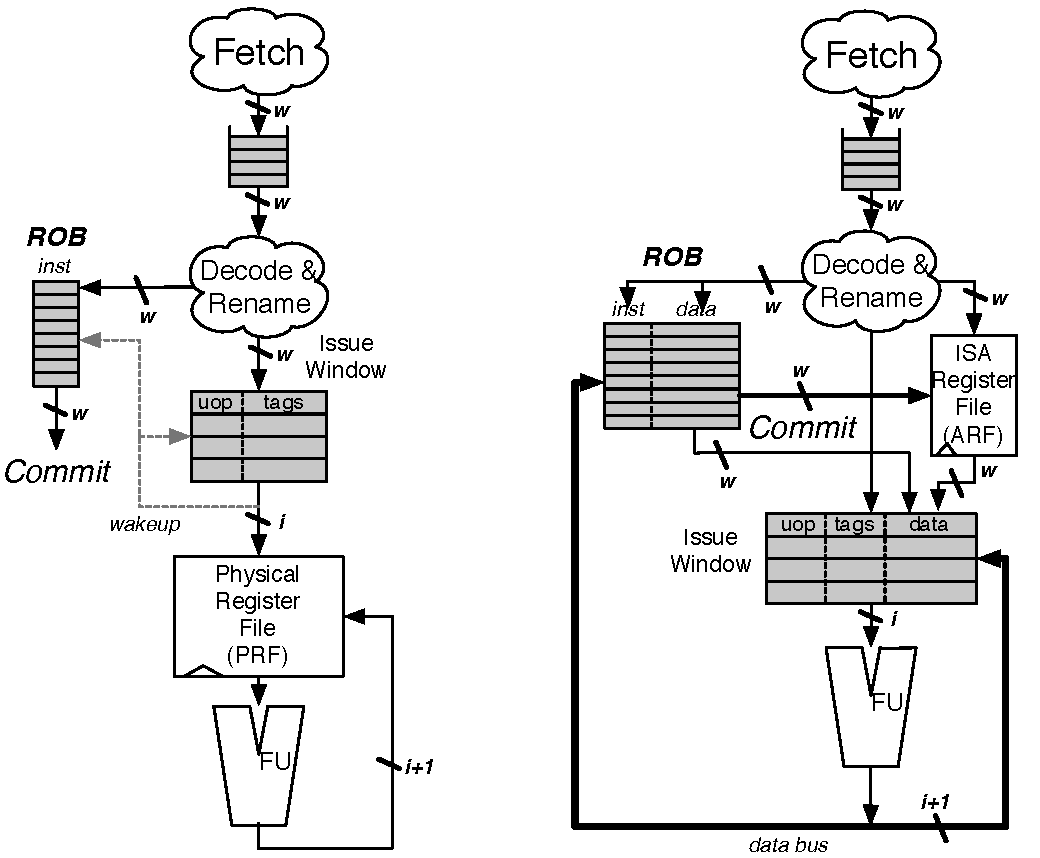
\includegraphics[scale =0.8] {figures/prf-and-arf}}
	\caption{ \small A PRF design (left) and a data-in-ROB design (right).}
	\label{fig:prf_design}
\end{figure}


This is in contrast to an ``implicit renaming" or ``data-in-ROB" out-of-order core design.  The Architectural Register File (ARF) only holds the committed register state, while the ROB holds the speculative write-back data.  On commit, the ROB transfers the speculative data to the ARF. 

The Pentium 4 and the ARM Cortex A57 are examples of {\em implicit renaming} designs.




\begin{figure}[htb]
	\centering
	\centerline{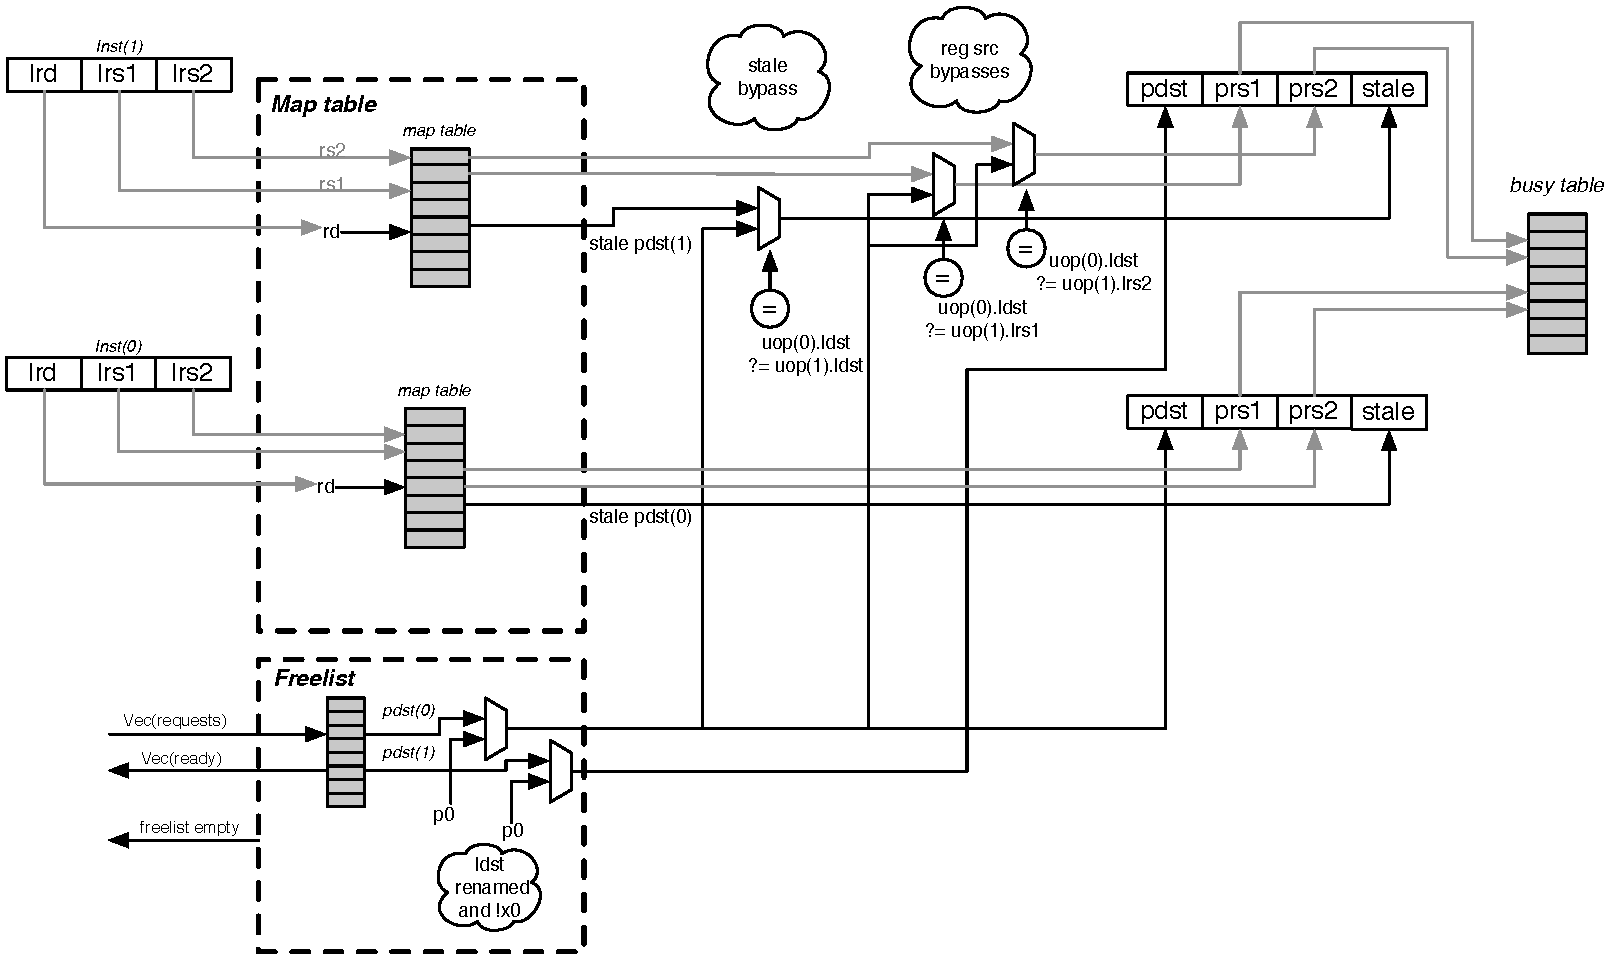
\includegraphics[scale =0.6] {figures/rename-pipeline}}
	\caption{ \small The Rename Stage. Logical register specifiers read the map table to get their physical specifier. For superscalar rename, any changes to the map tables must be bypassed to dependent instructions. The physical source specifiers can then read the Busy Table. The {\em Stale} specifier is used to track which physical register will be freed when the instruction later commits. P0 in the Physical Register File is always 0.}
	\label{fig:rename-pipeline}
\end{figure}


\section{The Rename Map Tables}

The Rename Map Tables hold the speculative mappings from ISA registers to physical registers.  

Each branch gets its own copy of the rename map tables.\footnote{An alternate design for wider pipelines may prefer to only make up to one snapshot per cycle, but this comes with additional complexity to deduce the precise mappings for any given instruction within the fetch packet.}  On a branch mispredict, the map table can be reset instantly from the mispredicting branch's copy of the map table. 

As the RV64G ISA uses fixed locations of the register specifiers (and no implicit register specifiers), the map tables can be read before the instruction is decoded!  

\subsection{Resets on Exceptions and Flushes}


An additional, optional ``Committed Map Table" holds the rename map for the committed architectural state.  If enabled, this allows single-cycle reset of the pipeline during flushes and exceptions (the current map table is reset to the committed map table). 


\section{The Busy Table}

The Busy Table tracks the readiness status of each physical register. If all physical operands are ready, the instruction will be ready to be issued. 

\section{The Free List}

The free-list tracks the physical registers that are currently un-used and is used to allocate new physical registers to instructions passing through the {\em Rename} stage.  

The Free List is implemented as a bit-vector.  A priority decoder can then be used to find the first free register. BOOM uses a cascading priority decoder to allocate multiple registers per cycle.\footnote{A two-wide rename stage could use two priority decoders starting from opposite ends.}

\section{Stale Destination Specifiers}

For instructions that will write a register, the map table is read to get the {\em stale physical destination specifier} (``stale pdst").  Once the instruction commits, the {\em stale pdst} is returned to the free list, as no future instructions will read it.

\chapter{The Issue Unit}

The issue window holds dispatched micro-ops that have not yet executed.  When all of the operands for the micro-op are ready, the issue slot sets its ``request" bit high.  The issue select logic then chooses to issue a slot which is asserting its ``request" signal.  Once a micro-op is issued, it is removed from the issue window to make room for more dispatched instructions. 

Future designs may choose to *speculatively* issue micro-ops (e.g., speculating that a load instruction will hit in the cache and thus issuing dependent micro-ops assuming the load data will be available in the bypass network). In such a scenario, the issue window cannot remove speculatively issued micro-ops until the speculation has been resolved. If a speculatively-issued micro-op failure occurs, 



\section{Issue Slot}

Figure \ref{fig:riscv-boom_issue_slot} shows a single issue slot from the {\em Issue Window}.\footnote{Conceptually, a bus is shown for implementing the driving of the signals sent to the {\em Register Read} Stage.  In reality BOOM actually uses muxes.}

Instructions (actually they are ``micro-ops" by this stage) are {\em dispatched} into the {\em Issue Window}.  From here, they wait for all of their operands to be ready (``p" stands for {\em presence} bit, which marks when an operand is {\em present} in the register file).  

Once ready, the {\em issue slot} will assert its ``request" signal, and wait to be {\em issued}.  Currently, BOOM only issues a single micro-op every cycle, and has a fixed priority encoding to give the lower ID entries priority.


\begin{figure}[ht]
	\centering
	\centerline{\includegraphics[scale =1.0] {figures/rv32_boom_issue_slot}}
	\caption{ \small A single issue slot from the Issue Window.}
	\label{fig:riscv-boom_issue_slot}
\end{figure}

\section{Issue Select Logic}



\section{Un-ordered Issue Window}

\section{Age-ordered Issue Window}


\chapter{The Load/Store Unit (LSU)}\label{sec:lsu}

The Load/Store Unit is responsible for deciding when to fire memory operations to the memory system.  There are three queues: the Load Address Queue (LAQ), the Store Address Queue (SAQ), and the Store Data Queue (SDQ).  Load instructions generate a ``uopLD" micro-op.  When issued, ``uopLD" calculates the load address and places its result in the LAQ.  Store instructions (may) generate {\em two} micro-ops,  ``uopSTA" (Store Address Generation) and ``uopSTD" (Store Data Generation).  The STA micro-op calculates the store address and places its result in the SAQ queue.  The STD micro-op moves the store data from the register file to the SDQ.  Each of these micro-ops will issue out of the {\em Issue Window} as soon their operands are ready.  See Section \ref{sec:storeuops} for more details on the store micro-op specifics. 

\subsection{Store Instructions}

Entries in the Store Queue\footnote{When I refer to the {\em Store Queue}, I really mean both the SAQ and SDQ.} are allocated in the {\em Decode} stage (the appropriate bit in the {\tt stq\_entry\_val} vector is set).  A ``valid" bit denotes when an entry in the SAQ or SDQ holds a valid address or data ({\tt saq\_val} and {\tt sdq\_val} respectively).  Once a store instruction is committed, the corresponding entry in the Store Queue is marked as committed.  The store is then free to be fired to the memory system at its convenience.  Stores are fired to the memory in program order.


\subsection{Store Micro-ops}\label{sec:storeuops}

Stores are inserted into the issue window as a single instruction (as opposed to being broken up into separate {\tt addr-gen} and {\tt data-gen} micro-ops). This prevents wasteful usage of the expensive issue window entries and extra contention on the issue port to the LSU.  A store in which both operands are ready can be issued to the LSU as a single micro-op which provides both the address and the data to the LSU.  While this requires store instructions to have access to two register file read ports, this is motivated by a desire to not cut performance in half on store-heavy code.  Sequences involving stores to the stack should operate at IPC=1!

However, it is common for store addresses to be known well in advance of the store data.  Store addresses should be moved to the SAQ as soon as possible to allow later loads to avoid any memory ordering failures. Thus, the issue window will emit uopSTA or uopSTD micro-ops as required, but retain the remaining half of the store until the second operand is ready.

\subsection{Load Instructions}

Entries in the Load Queue (LAQ) are allocated in the {\em Decode} stage ({\tt laq\_entry\_val}).  In {\em Decode}, each load entry is also given a {\em store mask} ({\tt laq\_st\_mask}), which marks which stores in the Store Queue the given load depends on.  When a store is fired to memory and leaves the Store Queue, the appropriate bit in the {\em store mask} is cleared.

Once a load address has been computed and placed in the LAQ, the corresponding {\em valid} bit is set ({\tt laq\_val}). 

Loads are optimistically fired to memory on arrival to the LSU (getting loads fired early is a huge benefit of out--of--order pipelines).  Simultaneously, the load instruction compares its address with all of the store addresses that it depends on.  If there is a match, the memory request is killed.  If the corresponding store data is present, then the store data is {\em forwarded} to the load and the load marks itself as having {\em succeeded}.  If the store data is not present, then the load goes to {\em sleep}.  Loads that have been put to sleep are woken at {\em Commit} time.\footnote{Higher performance processors will track {\em why} a load was put to sleep and wake it up once the blocking cause has been alleviated.}


\subsection{Memory Ordering Failures}

The Load/Store Unit has to be careful regarding {\tt store$\rightarrow$load} dependences.  For the best performance, loads need to be fired to memory as soon as possible. 

\begin{quote}

{\texttt
sw x1 $\rightarrow$ 0(x2)

ld x3 $\leftarrow$ 0(x4)
}

\end{quote}


However, if {\tt x2} and {\tt x4} reference the same memory address, then the load in our example {\em depends} on the earlier store.  If the load issues to memory before the store has been issued, the load will read the wrong value from memory, and a {\em memory ordering failure} has occurred.  On an ordering failure, the pipeline must be flushed and the rename map tables reset.  This is an incredibly expensive operation.

To discover ordering failures, when a store commits, it checks the entire LAQ for any address matches.  If there is a match, the store checks to see if the load has {\em executed}, and if it got its data from memory or if the data was forwarded from an older store.  In either case, a memory ordering failure has occurred.  

See Figure \ref{fig:lsu} for more information about the Load/Store Unit.

\


\begin{figure}[ht]
	\centering
	\centerline{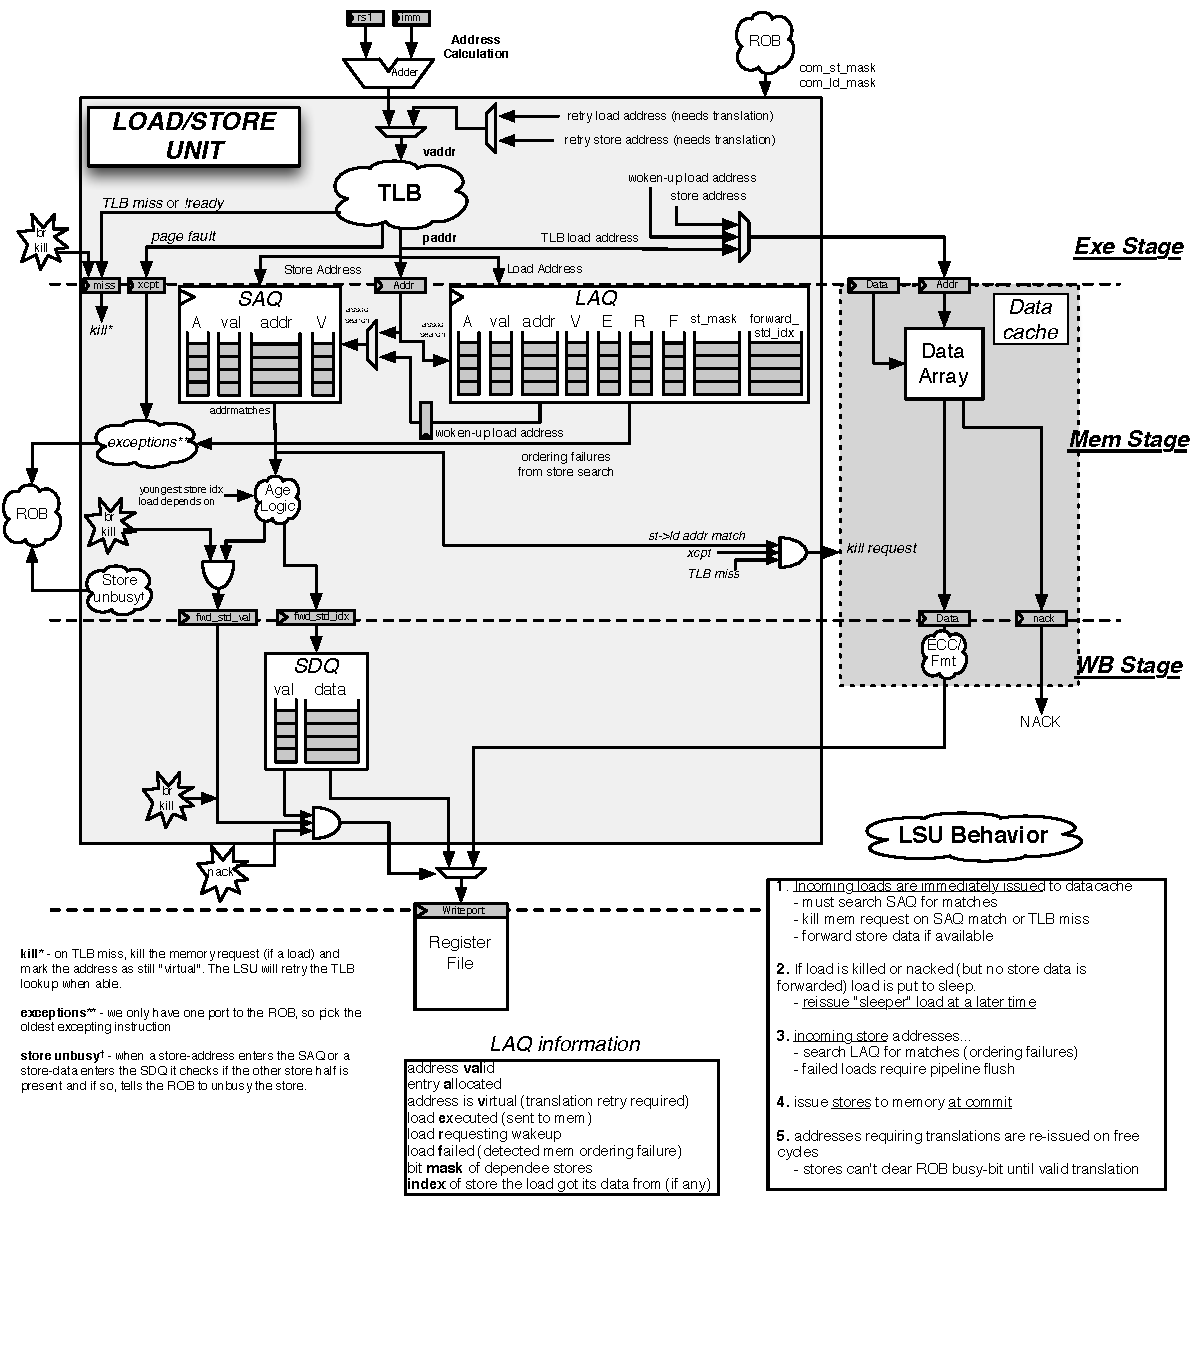
\includegraphics[scale =.9] {figures/lsu}}
	\caption{ \small The Load/Store Unit.}
	\label{fig:lsu}
\end{figure}


\chapter{The Memory System and the Data-cache Shim}

BOOM uses the Rocket non-blocking cache (``Hellacache").  Designed for use in in-order vector processors, a ``shim'' is used to connect BOOM to the data cache. The source code for the cache can be found in {\texttt nbdcache.scala} in the Rocket repository (\url{github.com/ucb-bar/rocket}). 

The contract with the cache is that it may execute all memory operations sent to it (barring structural hazards).  As BOOM will send speculative load instructions to the cache, the shim ({\texttt dcacheshim.scala})  must track all ``inflight load requests" and their status. If an inflight load is discovered to be misspeculated, it is marked as such in the shim.  Upon return from the data cache, the load's response to the pipeline is suppressed and it is removed from the inflight load queue. 

The Hellacache does not {\tt ack} store requests; the absence of a {\tt nack} is used to signal a success. 

All memory requests to the Hellacache may be killed the cycle after issuing the request (while the request is accessing the data arrays).  

The current data cache design accesses the SRAMs in a single-cycle. 

\chapter{The Reorder Buffer (ROB)}
\chapter{Micro-architectural Counters}

The current RISC-V gcc toolchain provides access to 16 named ``uarch" counters.\footnote{The future plan of record is to move these counters into the memory-mapped access region. This will open up the ability to track a much larger number of counters, as desired.}

\begin{table}[htdp]
\caption{Uarch Counters}
\begin{center}
\begin{tabular}{|c|c|}
\hline
Number & Event \\
\hline
\hline
0 & Committed Branch Mispredictions \\
\hline
1 & Committed Branches \\
\hline
\end{tabular}
\end{center}
\label{table:uarchcounters}
\end{table}%

The counters can be modified in {\tt dpath.scala} to track events of interest.

{\bf Note:} the counters can be quite large (64-bits each), and it is recommended that alternative methods be used if a silicon is the end-product. A design that can multiplex counters is recommended. 

\section{Reading UArch Counters in Software}

The Code Example \ref{ref:code_uarch} demonstrates how to read the value of any CSR register from software.
  
  
\begin{center}
\begin{minipage}{0.66\textwidth}
\begin{lstlisting}[caption=Reading a CSR register]
#define read_csr_safe(reg) ({ register long __tmp asm("a0"); \   
  asm volatile ("csrr %0, " #reg : "=r"(__tmp)); \               
  __tmp; })             
  
  long csr_cycle   = read_csr_safe(cycle);
  long csr_instr   = read_csr_safe(instret);
  long csr_uarch0  = read_csr_safe(uarch0);
  ...
  long csr_uarch15 = read_csr_safe(uarch15);
  
\end{lstlisting}\label{ref:code_uarch}
\end{minipage}
\end{center}





\chapter{Verification}

This chapter covers the current recommended techniques for verifying BOOM.  Although not provided as part of the BOOM or rocket-chip repositories, it is also recommended that BOOM be tested on ``hello-world + riscv-pk" and the RISC-V port of Linux to properly stress the processor.

\section{RISC-V Tests}

A basic set of functional tests and micro-benchmarks can be found at (\url{https://github.com/riscv/riscv-tests}).  These are invoked by the ``make run" targets in the emulator, fsim, and vsim directories. 

\section{RISC-V Torture Tester}

Berkeley's {\tt riscv-torture} tool is used to stress the BOOM pipeline, find bugs, and provide small code snippets that can be used to debug the processor. Torture can be found at (\url{https://github.com/ucb-bar/riscv-torture}).

\

\begin{quote}
{\bf Quick-start}

\texttt{\#} compile the BOOM C++ emulator

\texttt{\$} \verb=cd rocket-chip/emulator; make run CONFIG==\verb=BOOMCPPConfig=

\

\texttt{\#} check out and run the {\tt riscv-torture} repository

\texttt{\$} \verb=cd ../          # top-level rocket-chip directory=

\texttt{\$} \verb=git clone https://github.com/ucb-bar/riscv-torture.git=

\texttt{\$} \verb=cd riscv-torture=

\texttt{\$} \verb=git submodule update --init=

\texttt{\$} \verb=vim Makefile    # change RTL_CONFIG==\verb=BOOMCPPConfig=

\texttt{\$} \verb=make igentest   # test that torture works, gen a single test=

\texttt{\$} \verb=make cnight     # run C++ emulator overnight=
\end{quote}



\chapter{Debugging}





\appendix

\chapter{Future Work}

This chapter lays out some of the potential future directions that BOOM can be taken.  To help facilitate such work, the preliminary design sketches are described below. 

\section{The Rocket Custom Co-processor Interface (ROCC)}

The Rocket in-order processor comes with a ROCC interface that facilitates communication with co-processor/accelerators.  Such accelerators include crypto units (e.g., SHA3) and vector processing units (e.g., the open-source Hwacha vector-thread unit\cite{hwacha}). 

The ROCC interface accepts co-processor commands emitted by {\em committed} instructions run on the ``Control Processor" (e.g., a scalar Rocket core).  Any ROCC commands {\em will} be executed by the co-processor (barring exceptions thrown by the co-processor); nothing speculative can be issued over ROCC. 

Some ROCC instructions will write back data to the Control Processor's scalar register file. 

\subsection{The Demands of the ROCC Interface}


The ROCC interface accepts a ROCC command and up to two register inputs from the Control Processor's scalar register file. 
The ROCC command is actually the entire RISC-V instruction fetched by the Control Processor (a ``ROCC instruction"). Thus, each ROCC queue entry is at least 2*XPRLEN + 32 bits in size (additional ROCC instructions may use the longer instruction formats to encode additional behaviors). \TODO{draw a diagram showing this}

As BOOM does not store the instruction bits in the ROB, a separate data structure (A ``ROCC Reservation Station") will have to hold the instructions until the ROCC instruction can be committed and the ROCC command sent to the co-processor. 

The source operands will also require access to BOOM's register file.  Two possibilities are proposed:

\begin{itemize}
\item ROCC instructions are dispatched to the Issue Window, and scheduled so that they may access the read ports of the register file once the operands are available. The operands are then written into the ROCC Reservation Station, which stores the operands and the instruction bits until they can be sent to the co-processor.  This may require significant state. 
\item ROCC instructions, when they are committed and sent to the ROCC command queue, must somehow access the register file to read out its operands.  If the register file has dynamically scheduled read ports, this may be trivial. Otherwise, some technique to either inject a ROCC micro-op into the issue window or a way to stall the issue window while ROCC accesses the register file will be needed. 
\end{itemize}


\subsection{A Simple One-at-a-Time ROCC Implementation}

The simplest way to add ROCC support to BOOM would be to stall {\em Decode} on every ROCC instruction and wait for the ROB to empty.  Once the ROB is empty, the ROCC instruction can proceed down the BOOM pipeline non-speculatively, and get sent to the ROCC command queue.  BOOM remains stalled until the ROCC accelerator acknowledges the completion of the ROCC instruction and sends back any data to BOOM's register file. Only then can BOOM proceed with its own instructions. 


\subsection{A High-performance ROCC Implementation Using Two-Phase Commit}

While some of the above constraints can be relaxed, the performance of a decoupled co-processor depends on being able to queue up multiple commands while the Control Processor runs ahead (prefetching data and queueing up as many commands as possible).  However, this requirement runs counter to the idea of only sending committed ROCC instructions to the co-processor. 

BOOM's ROB can be augmented to track {\em commit} and {\em non-speculative} pointers. The {\em commit} head pointer tracks the next instruction that BOOM will {\em commit}, i.e., the instruction that will be removed from the ROB and the resources allocated for that instruction will be de-allocated for use by incoming instructions. The {\em non-speculative} head will track which instructions can no longer throw an exception and are no longer speculated under a branch (or other speculative event), i.e., which instructions absolutely will execute and will not throw a pipeline-retry exception. 

This augmentation will allow ROCC instructions to be sent to the ROCC command queue once they are deemed ``non-speculative", but the resources they allocate will not be freed until the ROCC instruction returns an acknowledgement.  This prevents a ROCC instruction that writes a scalar register in BOOM's register file from overwriting a newer instruction's writeback value, a scenario that can occur if the ROCC instruction commits too early, followed by another instruction committing that uses the same ISA register as its writeback destination. 


\subsection{The BOOM Custom Co-processor Interface (BOCC)}

Some accelerators may wish to take advantage of speculative instructions (or even out-of-order issue) to begin executing instructions earlier to maximize de-coupling.  Speculation can be handled by either by epoch tags (if in-order issue is maintained to the co-processor) or by allocating mask bits (to allow for fine-grain killing of instructions). 

\section{The Vector (``V") ISA Extension}

Implementing the Vector Extension in BOOM would open up the ability to leverage performance (or energy-efficiency) improvements in running data-level parallel codes (DLP).  While it would be relatively easy to add vector arithmetic operations to BOOM, the significant challenges lie in the vector load/store unit. 


\section{The Compressed (``C") ISA Extension}

This section describes how to approach adding the Compressed ISA Extension to BOOM.  The Compressed ISA Extension, or RVC  (\url{http://riscv.org/download.html#spec_compressed_isa}) enables smaller, 16 bit encodings of common instructions to decrease the static and dynamic code size.  ``RVC" comes with a number of features that are of particular interest to micro-architects:

\begin{itemize}
\item All 16b instructions map directly into a longer 32b instruction. 
\item 32b instructions have no alignment requirement, and may start on a half-word boundary.
\end{itemize}

\begin{figure}[ht]
	\centering
	\centerline{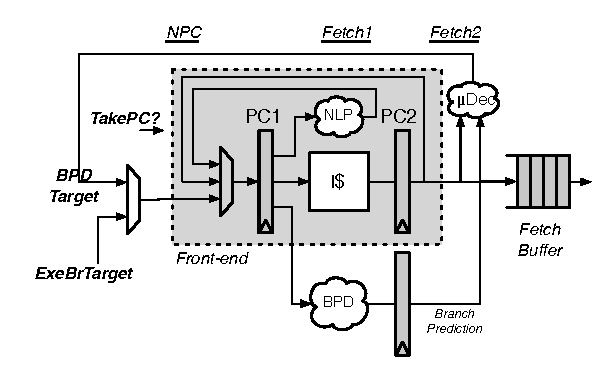
\includegraphics[scale =1] {figures/frontend}}
	\caption{ \small The Fetch Unit. The grey box encompasses the Rocket front-end, which is re-used by BOOM.}
	\label{fig:futurework-frontend}
\end{figure}

BOOM re-uses the front-end design from Rocket, a 5-stage in-order core.  BOOM then takes instructions returning (the {\em fetch packet}) from the Rocket front-end, quickly decodes the instructions for branch prediction, and pushes the {\em fetch packet} into the {\em Fetch Buffer}. 


The C Extension provides the following challenges to micro-architects, a few include:

\begin{itemize}
\item Increased decoding complexity (e.g., operands can now move around). 
\item Finding {\em where} the instruction begins. 
\item Tracking down $+4$ assumptions throughout the code base, particularly with branch handling.
\item Unaligned instructions, in particular, running off cache lines and virtual pages. 
\end{itemize}

The last point requires some additional ``statefulness" in the Fetch Unit, as fetching all of the pieces of an instruction may take multiple cycles. 

The following describes the proposed implementation strategy of RVC in BOOM:

\begin{itemize}
\item Implement RVC in the Rocket in-order core.  Done properly, BOOM may then gain RVC support almost entirely for free (modulo any $+4$ assumptions in the code base).
\item Move BOOM's {\em Fetch Buffer} into Rocket's front-end. Rocket will need the statefulness to handle wrap-around issues with fetching unaligned 32 bit instructions.  A non-RVC Rocket core can optionally remove this buffer. 
\item Expand 16-bit instructions as they enter (or possibly exit) the {\em Fetch Buffer}. 
\item Minimize latency by placing 16b$\rightarrow$32b expanders at every half-word start. 
\end{itemize}

\subsection{Challenging Implementation Details}

There are many challenging corner cases to consider with adding RVC support to BOOM. First, although all 16 bit encodings map to a 32b version, {\bf the behavior of some 16b instructions are different from their 32b counterparts}!  A JAL instruction writes the address of the following instruction to {\tt rd} - but whether that is $PC+2$ or $PC+4$ depends on whether it's the 16b JAL or a 32b JAL!  Likewise, a mispredicted not-taken branch redirects the fetch unit to $PC+2$ or $PC+4$ depending on whether the branch was the compressed version or not. {\bf Thus, the pipeline must track whether any given instruction was originally a compressed 16b instruction or not.}

The branch prediction units will also require a careful rethink. The BTB tracks which instructions are {\em predicted-taken} branches and redirects the PC as desired. For a superscalar {\em fetch packet}, the BTB must help denote which instruction is to be blamed for the taken prediction to help mask off any invalid instructions that come afterward within the {\em fetch packet}. RVC makes this much more difficult, as some {\em predicted-taken} branches can wrap around fetch groupings/cache lines/virtual page boundaries. Thus, the ``taken" prediction must be attached to a tag-hit on the {\em end} of the branch instruction.  This handles fetching the first part of the branch (and predicting ``not-taken"), then fetching the second part (which hits in the BTB and predicts ``taken"), and only then redirecting the front-end to the predicted-taken PC target. 

%TODO is this a problem?
%One final detail to keep in mind is the potential interactions of the i-cache and the instruction translation look-aside buffer (i-TLB) with regards to self-modifying RVC code.  A RISC-V instruction can legally straddle a virtual page boundary such that the second half is neither in the i-cache nor in the i-TLB. A self-modifying program could store out new instructions that are not resident in the i-cache (or i-TLB).  However, such a store could override the last half 


\chapter{Frequently Asked Questions}

To be filled in as questions are asked!


\chapter{Terminology}

To be filled in as needed.



\begin{figure}[ht]
	\centering
	\centerline{\includegraphics[scale =.9, angle=90] {figures/boom_detailed}}
	\caption{ \small A more detailed diagram of BOOM, for a single-issue RV32IM design.}
	\label{fig:boom-detailed}
\end{figure}






%\begin{scriptsize}
\bibliographystyle{abbrv}
\bibliography{bibliography}
%\end{scriptsize}


\end{document}
